\documentclass[10pt]{article}

\usepackage[letterpaper,left=0.75in,right=0.75in,top=0.64in,bottom=0.64in]{geometry}
\usepackage{graphicx}
\usepackage{microtype}
\usepackage{xcolor}
\usepackage{enumitem}
\usepackage{caption}
\usepackage{newtxtext,newtxmath}
\graphicspath{{figures/}{abstract/figures/}}

\pagestyle{empty}
\setlength{\parindent}{0pt}
\setlength{\parskip}{2.5pt}
\setlist{nosep,leftmargin=1.25em}
\captionsetup{font=small,labelfont=bf,skip=2pt}

\begin{document}

\begin{center}
{\Large\bfseries Do Visual Emotion Models Reason with the Cues They Report? A Counterfactual Audit of Cue-Aware Affective Reasoning}
\end{center}
\vspace{-0.45em}

\textbf{Motivation.}
Visual emotion systems increasingly accompany categorical or dimensional predictions with saliency, cue weights, or natural-language evidence. Yet agreement with image-level annotations does not establish that these reports describe the evidence controlling the output. A system may predict sadness from dark colour or background correlations while naming a face as justification. Recent VLM benchmarks similarly report intensity-calibration errors and shallow affective descriptions~[1], but output quality alone cannot establish evidence use. We therefore ask: \emph{do the cues a model reports agree with the cues to which its prediction is behaviourally sensitive?}

\textbf{Counterfactual Affective Twins.}
We make this question executable with a report-conditioned audit. First, the target model predicts emotion and valence--arousal from the untouched image, names its strongest cue family, and gives a short visible-evidence phrase. Second, the same model grounds that report to one candidate region supplied by independent segmentation, facial landmarks, or OCR. Only this reported evidence is manipulated to form the target ``twin'': colour or lighting over a complete semantic region, an AU-related brow, eye, or mouth region, subject-preserving scene context, or text already present in the image. Third, the same target model is run on the twin. We compare its response with an unreported-cue intervention and, when available, a mask-area-matched region from the reported cue family. A report is behaviourally faithful when changing the reported target alters the model more than these controls; invalid or ungroundable reports are counted as audit failures rather than replaced by a post-hoc salient region. This separates \emph{what a model says it used} from \emph{what controls its prediction}.

\begin{figure}[h]
    \centering
    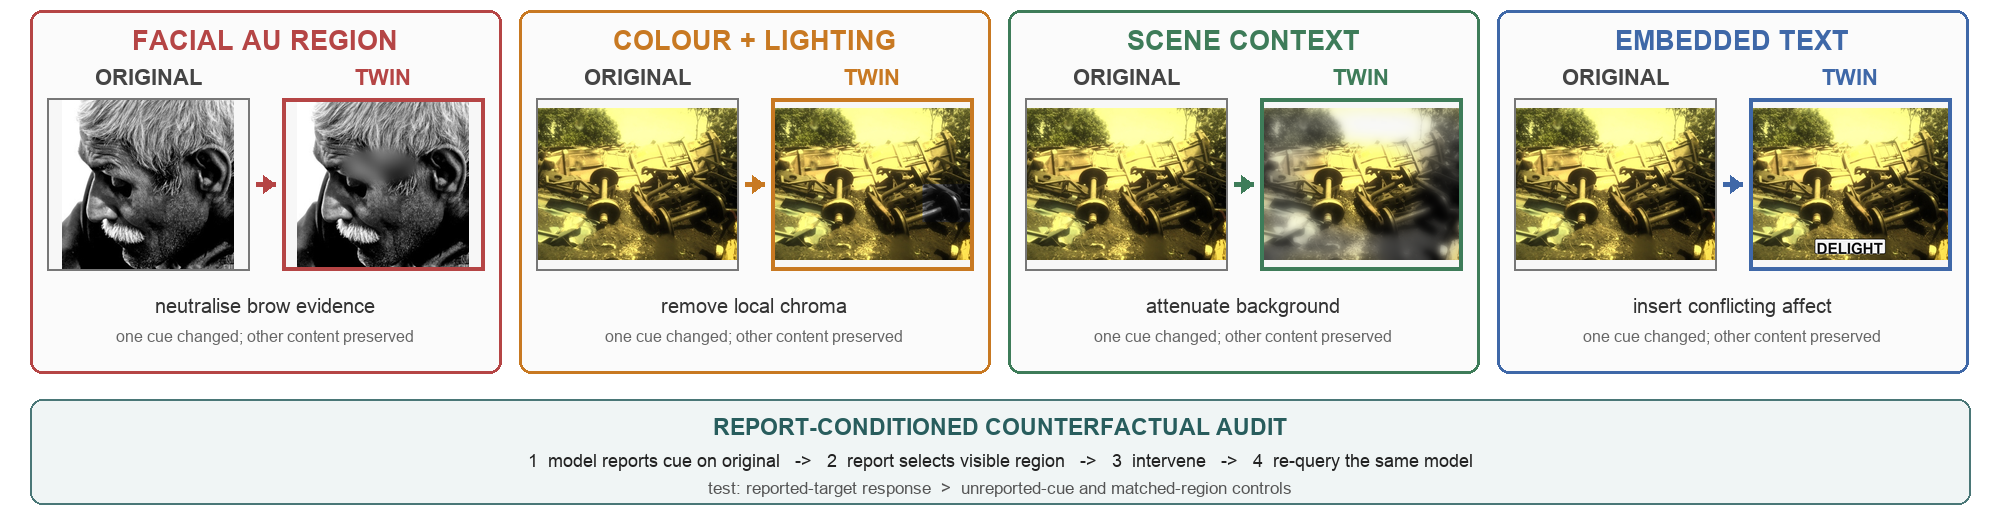
\includegraphics[width=\linewidth]{counterfactual_twins_examples.png}
    \caption{Implemented candidate interventions for the four reportable cue families. For each image, the model's pre-intervention report selects one family and one visible region; the resulting twin is then returned to the same model.}
    \label{fig:framework}
\end{figure}
\vspace{-0.55em}

\textbf{Feasibility study.}
We first test a necessary safeguard: does an affect-sensitive intervention selected by one model transfer to an independently fitted evaluator, or merely exploit the locator? Emotion6 contains 1,980 images collected under six affective retrieval categories and provides separate viewer-response distributions~[2]. In this initial category-supervised pilot, we train two emotion heads over frozen ImageNet-pretrained ResNet-18 features~[3] with independent initialisation and bootstrap samples; the evaluator obtains $51.7\%$ accuracy and $0.512$ macro-F1 on the 402-image test split. For 60 balanced held-out images, the locator ranks 16 equal-area regions by the reduction in retrieval-category probability after luminance-preserving chroma removal. The evaluator then assesses the selected region against all 15 area-matched controls. Selected interventions reduce retrieval-category probability by $0.070$, compared with $-0.001$ for controls. The paired advantage is $0.071$ (95\% bootstrap CI $[0.050,0.096]$) and is positive for 58 of 60 images. Thus, the detected colour sensitivity transfers across independently fitted heads rather than remaining a locator-specific saliency artefact.

\textbf{From feasibility to benchmark.}
The executable framework now stores the original report before generating any target twin, exact edit masks, the report-to-region decision, matched controls, and pre/post outputs. Its primary endpoints are prediction flips and reported-target minus control sensitivity; probability changes from the compact VLM are treated only as ordinal confidence proxies. Human raters separately verify edit naturalness, target-cue change, and preservation of non-target content before a pair is interpreted as a perceptual counterfactual. The audit therefore does not assume that a plausible explanation is causal. It tests the narrower and falsifiable claim that evidence named by a model should have greater behavioural influence than comparable evidence it did not name.

\vspace{0.1em}
{\footnotesize\textbf{References.}
[1] D. She et al. ``AICA-Bench: Holistically Examining the Capabilities of VLMs in Affective Image Content Analysis.'' \emph{Findings of ACL}, 2026.
[2] K.-C. Peng et al. ``A Mixed Bag of Emotions: Model, Predict, and Transfer Emotion Distributions.'' \emph{CVPR}, 2015.
[3] K. He et al. ``Deep Residual Learning for Image Recognition.'' \emph{CVPR}, 2016.}

\end{document}
